\documentclass{article}
\usepackage{homework}
\usepackage{amsmath}
\usepackage{amsthm}
\usepackage{listings}
\usepackage{graphicx}
\newcommand{\ea}[1]{\begin{eqnarray*}#1\end{eqnarray*}}
\newcommand{\leftbrace}[1]{\left\{\begin{array}{ll}#1 \end{array}\right.}

\author{Roman Stanchak}
\title{Homework I}
\begin{document}
\maketitle
\problem{1} Prove the Vandermonde matrix is nonsingular by showing that its determininant is nonzero.
\solution{1} In order to prove the Vandermonde matrix is nonzero, it will be shown that the determinant
takes a particular form.  If $A_n$ is the Vandermonde matrix for $n+1$ interpolation points,
\[
	|A_n| = (-1)^n\prod_{i=0}^{n}\prod_{j=i+1}^{n}(x_i-x_j)
\]
By this proposition, $|A_n|=0$ if and only if $x_i=x_j$ for some $i,j$.  However, the Vandermonde 
matrix by definiton is contructed of unique $x_i$'s, so this can not be the case, and therefore
$|A_n|\ne 0$.\\
\\
Proof of the proposition by induction on the number of interpolation nodes.
\begin{proof}[Base Case] Prove for $n=1$, $x_0,x_1$.\\
\ea{
	|A_1| &=& \left|
				  \begin{array}{cc} 1 & x_0 \\
		                            1 & x_1 
				  \end{array}
			 \right| \\
          &=& (x_1-x_0)
}
\end{proof}
\begin{proof}[Inductive Case] Assume for $n-1$ (i.e. $n$ interpolation nodes), prove for $n$ (i.e. $n+1$ interpolation nodes).\\
\ea{
	|A_n| &=& \left|
				\begin{array}{ccccc} 1 & x_0 & x_0^2 & \dots & x_0^n \\
					\dots \\
					\dots \\
					1 & x_n & x_n^2 & \dots & x_n^n
				\end{array}
			\right| \\
	&=& x_0^n|A_{n/0}| - x_1^n|A_{n/1}| + \dots + x_j^n|A_n{n/j}| + \dots + x_n^n|A_{n-1}|
}
Where $A_{n/j}$ is the determinant of the cofactor matrix excluding the $j$th 
row and $n$th column. Since the order of the points $x_0\dots x_n$ is arbitrary, 
and each of the $A_{n/j}$ cofactor matrices is size $n\times n$, the IH holds:
\ea{
	|A_n| &=& \sum_{i=0}^{n} x_i^n (-1)^n\prod_{j=0,j\ne i}^{n}\prod_{k=j+1}^{n}(x_j-x_k)
}
\textit{Don't know how to get from A to B}

\ea{
	|A_n| &=&  (-1)^n\prod_{i=0}^{n}\prod_{j=i+1}^{n} (x_i-x_j)
}
\end{proof}

\problem{2.}
Propose a method for finding the root $t^*$ of a function $g(t)$, where it is known that in the 
neighborhood of $t*$, $g$ has an inverse that is a degree $n$ polynomial, that is:
\[
	p_n(g(t))=t
	\]
for all $t$ near $t^*$.
\solution{2.}
The method should go something as follows:\\
Let $[a,b]$ be the interval consisting of the 'neightborhood' of $t^*$.  Choose 
$n+1$ distinct points $t_0,t_1,\dots,t_n$ from the interval and compute $g(t_j)$ for 
each.  Let $y_j=g(t_j)$. Since $g(t)$ has an inverse in the interval $[a,b]$, then the $y_j$'s are 
distinct.  $p_n(y)$ is then the interpolating polynomial for the interpolation nodes 
$y_0,y_1,\dots,y_n$ and interpolation data $t_0,t_1,\dots,t_n$.  The root $t^*$ is found simply by
evaluating $p_n(0)$.

\problem{3.}
Prove the formula:
$$f[x_0,x_1,\cdots,x_n] = \sum_{i=0}^{n} f(x_i) \prod_{j=0,j\neq i}^{n} (x_i - x_j)^{-1}$$
\solution{3.}
\begin{proof}
	Proof by induction on number of interpolation points.
	\begin{proof}[Base Case] Prove for $n=1$, $x_0,x_1$.\\
	Using the divided difference formula:
	\begin{eqnarray*}
	f[x_0,x_1]&=&\frac{f[x_1]-f[x_0]}{(x_1-x_0)}\\
	&=&\frac{f(x_1)-f(x_0)}{(x_1-x_0)}\\
	&=&\frac{f(x_0)}{x_0-x_1}+\frac{f(x_1)}{(x_1-x_0)}\\
	&=&\sum_{i=0}^{1}f(x_i)\prod_{j=0,j\neq i}^{1} (x_i - x_j)^{-1}
	\end{eqnarray*}
	\end{proof}
	\begin{proof}[Inductive Case] Assume that for $\forall k<n$ points, the formula holds.  Prove for $n$ points.\\
	Again using the divided difference formula:
	\begin{eqnarray*}
		f[x_0,x_1,\cdots,x_n] &=& 
			\frac{ f[x_1,x_2,\cdots,x_n] - f[x_0,x_1,\cdots,x_{n-1}] }
			     { (x_n-x_0) }\\
	\end{eqnarray*}
	Since the ordering of the points and summation indices is arbitrary, and the
	terms $f[x_1\cdots x_n]$ and $f[x_0\cdots x_{n-1}]$ have fewer than $n$ points,
	the IH applies, and the following is true:
	\begin{eqnarray*}
		&=& \frac{\sum_{i=1}^{n} f(x_i) \prod_{j=1,j\neq i}^{n} (x_i - x_j)^{-1} 
		        - \sum_{i=0}^{n-1} f(x_i) \prod_{j=0,j\neq i}^{n-1} (x_i - x_j)^{-1}}
		         { (x_n-x_0) } \\
		&=& \sum_{i=1}^{n} \frac{f(x_i)}{(x_n-x_0) \prod_{j=1,j\neq i}^{n} (x_i - x_j)} - 
		    \sum_{i=0}^{n-1} \frac{f(x_i)}{(x_n-x_0) \prod_{j=0,j\neq i}^{n-1} (x_i - x_j)} \\
		&=& \frac{f(x_0)}{(x_n-x_0)\prod_{j=1,j\neq n}^{n} (x_n - x_j)} - 
		    \frac{f(x_n)}{(x_n-x_0)\prod_{j=0,j\neq 0}^{n-1} (x_0 - x_j)} + \Phi\\
		&=& \frac{f(x_0)}{\prod_{j=0,j\neq n}^{n} (x_n - x_j)} + 
		    \frac{f(x_n)}{\prod_{j=0,j\neq 0}^{n} (x_0 - x_j)} + \Phi\\
		\textrm{Where:} \\
		\Phi &=& 
			\sum_{i=1}^{n-1} \frac{f(x_i)}{(x_n-x_0) \prod_{j=1,j\neq i}^{n} (x_i - x_j)} -
			\sum_{i=1}^{n-1} \frac{f(x_i)}{(x_n-x_0) \prod_{j=0,j\neq i}^{n-1} (x_i - x_j)} \\
			&=& \sum_{i=1}^{n-1} \frac{f(x_i)}{ (x_n-x_0) \prod_{j=1,j\neq i}^{n-1} (x_i - x_j)}
				\left( \frac{1}{ (x_i - x_n) } - \frac{1}{ (x_i - x_0) } \right)\\
			&=& \sum_{i=1}^{n-1} \frac{f(x_i)}{ (x_n-x_0) \prod_{j=1,j\neq i}^{n-1} (x_i - x_j)}
				\cdot \frac{(x_i - x_0) - (x_i - x_n)}{ (x_i - x_n)(x_i - x_0) } \\
			&=& \sum_{i=1}^{n-1} \frac{f(x_i)}{ (x_n-x_0) \prod_{j=1,j\neq i}^{n-1} (x_i - x_j)}
				\cdot \frac{(x_n - x_0)}{ (x_i - x_n)(x_i - x_0) } \\
			&=& \sum_{i=1}^{n-1} \frac{f(x_i)}{ \prod_{j=0,j\neq i}^{n} (x_i - x_j)} \\
		\textrm{Substituting $\Phi$ back in above:}\\
		&=& \frac{f(x_0)}{\prod_{j=0,j\neq n}^{n} (x_n - x_j)} + 
		            \frac{f(x_n)}{\prod_{j=0,j\neq 0}^{n} (x_0 - x_j)} +
					\sum_{i=1}^{n-1} \frac{f(x_i)}{ \prod_{j=0,j\neq i}^{n} (x_i - x_j)} \\
		f[x_0,x_1,\cdots,x_n] &=& \sum_{i=0}^{n} f(x_i) \prod_{j=0,j\neq i}^{n} (x_i - x_j)^{-1}
	\end{eqnarray*}
\end{proof}
Thus, by the theory of induction, the proposition holds for $\forall n$.
\end{proof}
%%%%%%%%%%%%%%%%%%%%%%%%%%%%%%%%%%%%%%%%%%%%%%%%%%%%%%%%%%%%%%%%%%%%%%%%%%%%%%%
\problem{4} Given distinct points $x_0 \dots x_n$, the value of polynomial 
$p(x)$ at each, $f_j=p(x_j)$, and the value of the deriviative at each, 
$f_j'=p'(x_j)$, represent the interpolating polynomial as:
\[
	p(x) = \sum_{j=0}^n f_j\alpha_j(x) + \sum_{j=0}^n f_j'\beta_j(x)
\]
\solution{a}The requirements on $\alpha$ and $\beta$ are as follows:\\
\ea{
	\alpha_j(x) &=& \leftbrace{ 1 & x=x_j \\
	                         0 & \textrm{otherwise}
							} \\
	\alpha_j'(x) &=& 0, \forall x_j \\
	\beta_j(x) &=& 0, \forall x_j \\
	\beta_j'(x) &=& \leftbrace{ 1 & x=x_j \\
	                            0 & \textrm{otherwise}
							}
}
\solution{b} Given the $n+1$ points and the values of $p(x)$ and $p'(x)$ for each, amounts to
$2(n+1)$ constraints on the coefficients of the polynomial. This corresponds to a $2n+1$ degree
polynomial. Writing out the constraints for each point in matrix form:
\ea{
	\left[ \begin{array}{ccccc} 
			  1 & x_0 & x_0^2 & \dots & x_0^n \\
			  0 & 1   & 2\cdot x_0 & \dots & n\cdot x_0^{n-1} \\
			  1 & x_1 & x_1^2 & \dots & x_1^n \\
			  0 & 1   & 2\cdot x_1 & \dots & n\cdot x_1^{n-1} \\
			  \dots \\
			  1 & x_n & x_n^2 & \dots & x_n^n \\
			  0 &  1  & 2\cdot x_n & \dots & n\cdot x_n^{n-1}
			\end{array}
	\right]
	\left[ \begin{array}{c}
		\alpha_0\\
		\alpha_1\\
		\dots \\
		\alpha_{2n+2}
	\end{array}\right]
	&=& 
	\left[ \begin{array}{c}
		f(x_0) \\
		f'(x_0) \\
		f(x_1) \\
		f'(x_1) \\
		\dots \\
		f(x_n) \\
		f'(x_n) 
	\end{array}\right]
}
Based on my experiments with a CAS with n=1, it is possible that\dots\\
\ea{
\alpha_i(x) &=& l_i^2(x)l_i'(x) \\
	\beta_i(x) &=& ?
}

\problem{5} Given distinct $x_0,x_1,\dots,x_n$, and $y_0,y_1,\dots,y_n$, we seek the function:
	\[
		p_n(x) = \sum_{j=0}^n c_je^{jx}
	\]
	such that $p_n(x_j)=y_j$. Show there is a unique choice of $c_j$ for which this is true.
\solution{5}
\begin{proof}
Each $x_j,y_j$ provides a constraint on the linear system of equations consisting of the $c_j$'s:
\[
	y_j = \sum_{i=0}^n c_i e^{ix_j}
\]
Let $z_j=e^{x_j}$.  As a result,
\[
	y_j = \sum_{i=0}^n c_i z_j^i
\]
This is just the standard polynomial interpolation problem for which there exists a unique set of
$c_j$'s if $z_j$'s are unique.  $x_j$'s as given are unique. Thus, $z_j=e^x_j$ is also unique because $e^x$ is 
a strictly increasing function.  As a result, there exists a unique set of $c_j$'s as proposed.
\end{proof}
\problem{6a.}
\solution{6a.}
See Figure~\ref{fig:src1} for source code.

%---------------------------------------------------------------
\lstset{language=matlab}
%\lstset{backgroundcolor=listinggray,framerulecolor=blue}
%\lstset{backgroundcolor=listinggray,rulecolor=blue}
%\lstset{backgroundcolor=\color{listinggray},rulecolor=\color{blue}}
\lstset{linewidth=\textwidth}
%\lstset{labelstep=10}
%\lstset{commentstyle=\textit, stringstyle=\upshape,stringspaces=false}
\lstset{commentstyle=\textit, stringstyle=\upshape,showspaces=false}
\lstset{frame=trBL,frameround=tttt}
%\lstinputlisting[caption=Some MATLAB Code,label=lst:lowertri]{lowertri.m}
%---------------------------------------------------------------
\begin{figure}[htb]
	\lstinputlisting{newton_poly.m}
	\caption{Listing from source file \texttt{newtonpoly.m}}
	\label{fig:src1}
\end{figure}

\solution{6b.} See Figure~\ref{fig:src2} for source code and Figures~\ref{fig:fx1}~and~\ref{fig:fx2} for 
function graphs.
\begin{figure}[htb]
	\lstinputlisting{eval_newton.m}
	\caption{Listing from source file \texttt{newtoneval.m} }
	\label{fig:src2}
\end{figure}
\begin{figure}[htb]
	\begin{center}
		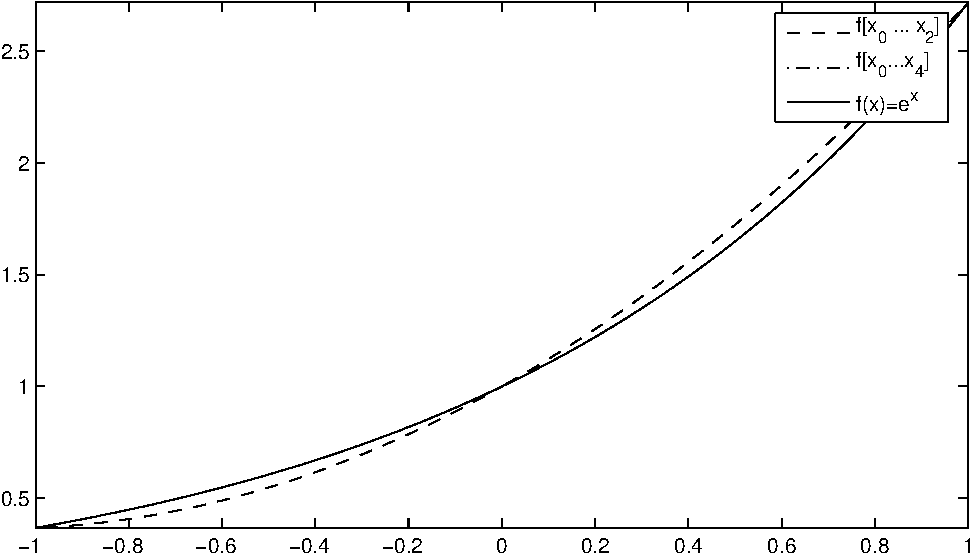
\includegraphics{newton_fx1-crop}	
	\end{center}
	\caption{Plot of $e^x$ and $p(x)$ interpolated at 3 and 5 points.}
	\label{fig:fx1}
\end{figure}
\begin{figure}[hb]
	\begin{center}
		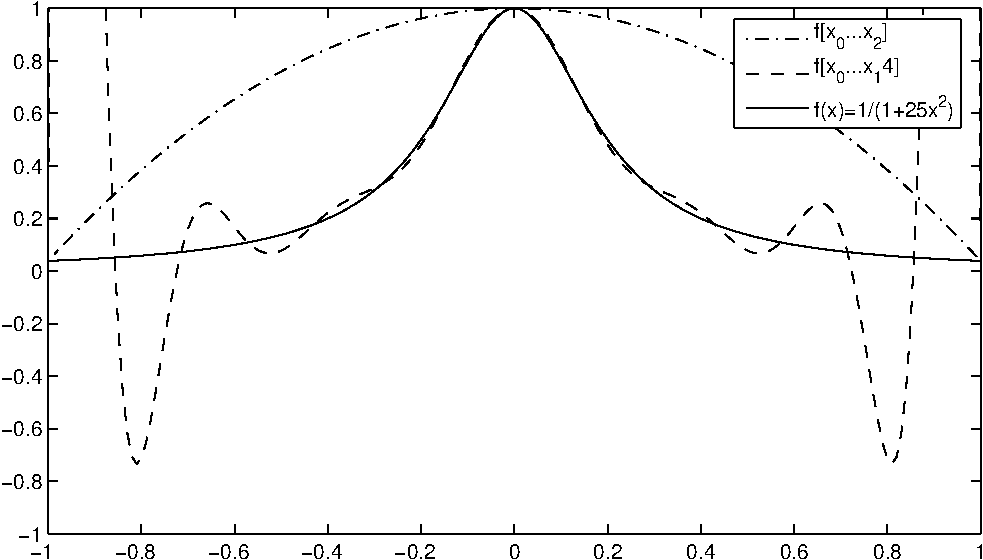
\includegraphics{newton_fx2-crop}	
	\end{center}
	\caption{Plot of $\frac{1}{1+25x^2}$ and $p(x)$ interpolated at 3 and 15 points.}
	\label{fig:fx2}
\end{figure}
\end{document}
